\subsection{Data Visualization Research}
With the field of soundscape ecology being a relatively new one, the format of data visualizations is not yet cemented in the community. In addition to the basic functionality of analyzing sound data for metrics, another goal of this project is to research and define useful visualizations for both researchers and data consumers. Each index provides a different method of analyzing natural soundscapes, so not all forms of data representations will apply to each. The goal of this section is to shed light on the reasoning behind the decisions to use each index\textquotesingle s respective visualization in the service.

\subsubsection{Outlier Identification}
An important part of the analysis of the sound files is to identify when outliers arise. Our sponsor has expressed that being able to see when an outlier occurs and being able to listen to what caused it is important in drawing conclusions and finding interesting bits of information from a data set. Thus, two infographics seem reasonable, those being timelines and line charts. Both do relatively similar jobs, however a timeline is made specifically for information over time. The only upside to a line graph would be that each point on the graph would represent a sound file, and the results of its analysis. Being able to represent an output as a small dot on a chart and allowing the user to select or hover over that point to see which file caused the outlier is certainly desirable from a usability perspective. Implementing a full-fledged sound file analysis section seems a bit out of scope for this project, so a line graph used to represent each sound file in a data set and the results of each file\textquotesingle s analysis is the best way to help the user identify outliers in the data.\par

\begin{center}
  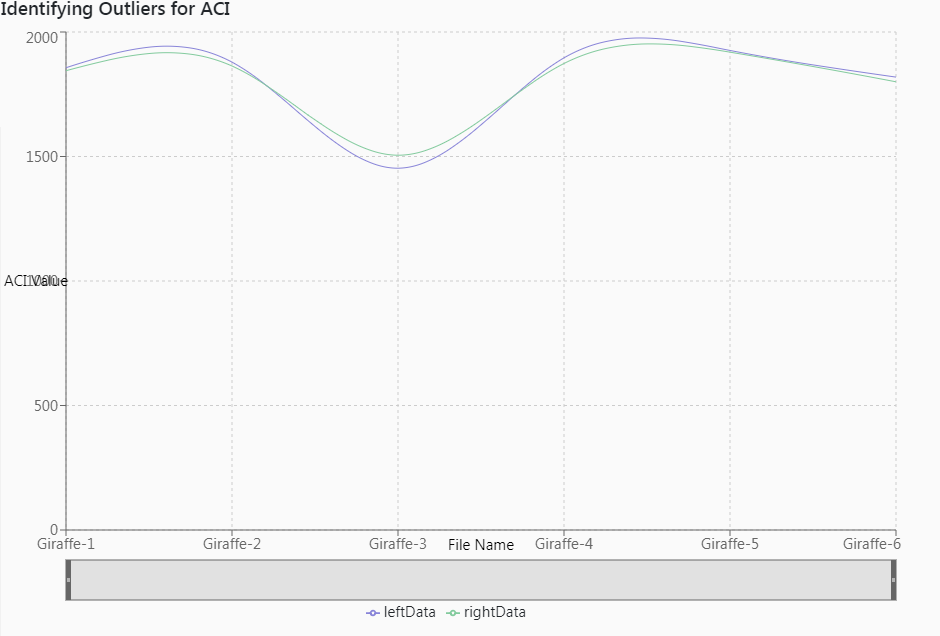
\includegraphics[width=\textwidth]{OutlierACIgraph1} \\[12pt]
  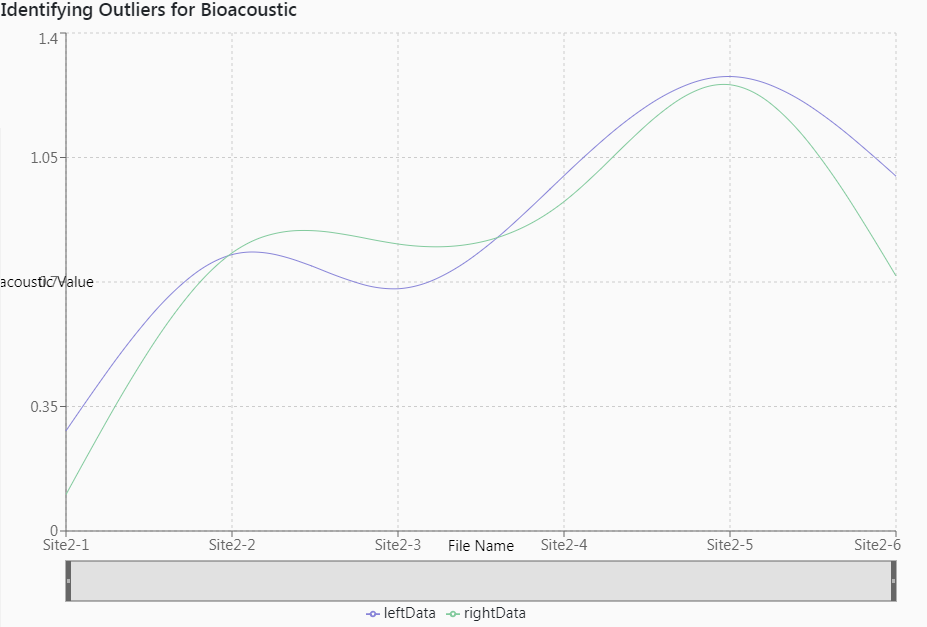
\includegraphics[width=\textwidth]{OutlierBAgraph1} \\[12pt]
\end{center}
The graphs above are for a data set comprised of files that the ACI and Bioacoustic Index was run on. The X axis displays the file name, while the Y axis labels the respective index value. Notice that file Giraffe 3 is much lower than the rest in the first graphic, and the file Site2-1 and Site2-5 also stand out in the second. Using these visuals, a researcher can quickly identify which files in their sets contain possibly interesting sounds to listen to in order to make further conclusions about their data.

\subsubsection{NDSI Visualization}
The NDSI index measures the relationship between the biophony and the anthrophony of a recording. This is elaborated on in the Overview of Indices section of this report. Because the NDSI is used for comparing two different variables, the representation for this index is different from that of ACI or ADI. Here, two bar charts have been chosen: one for comparing the values per channel, and another for comparing the values side by side. In addition, two line graphs are available for observing the NDSI values along with the biophony and anthrophony for data sets comprised of multiple files, and for analyzing these values at their respective date and time.\par

\begin{center}
  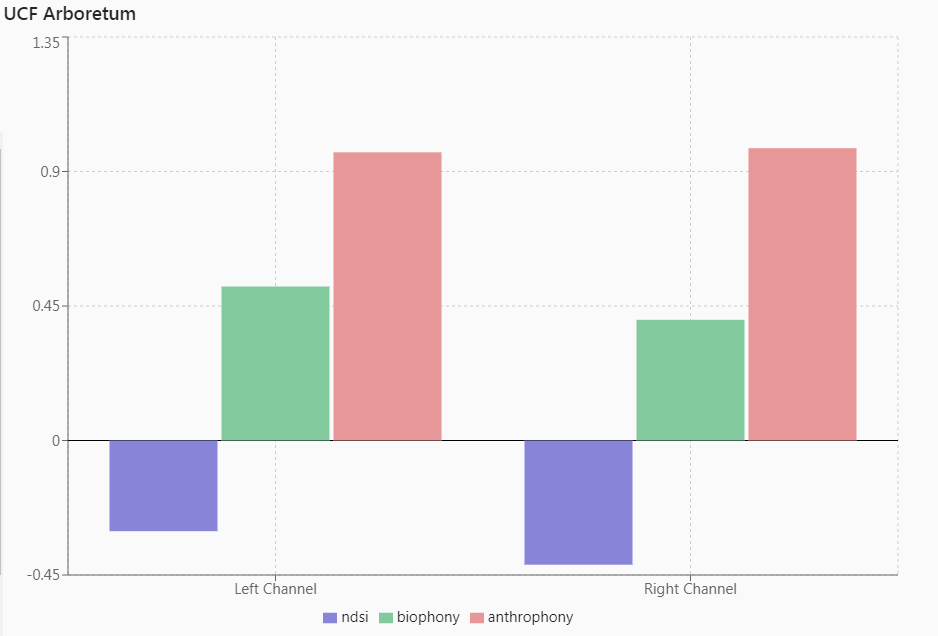
\includegraphics[width=\textwidth]{NDSIgraph1} \\[12pt]
\end{center}
The first visualization available is a bar graph comparing the two channels. Each channel has an overall NDSI value, along with biophony and anthrophony values. Because the NDSI is a difference of the anthrophony and biophony, it is useful to view them side by side in this way. The user is also able to hover over any bar and see the respective data values as they please.\par

\begin{center}
  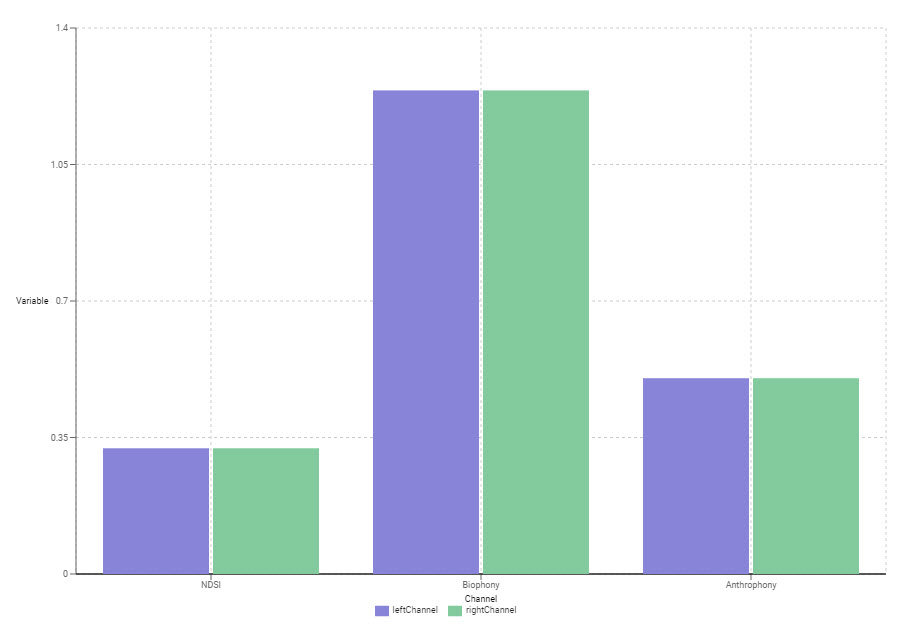
\includegraphics[width=\textwidth]{NDSIgraph2} \\[12pt]
\end{center}
The other visualization available is another bar graph, this one showing the NDSI values, anthrophony values, and biophony values side by side, sorted by channel this time. This representation is useful because often times one channel of the microphone gets different data than the other, and so being able to identify which channel has these differences is helpful for research.\par

\begin{center}
  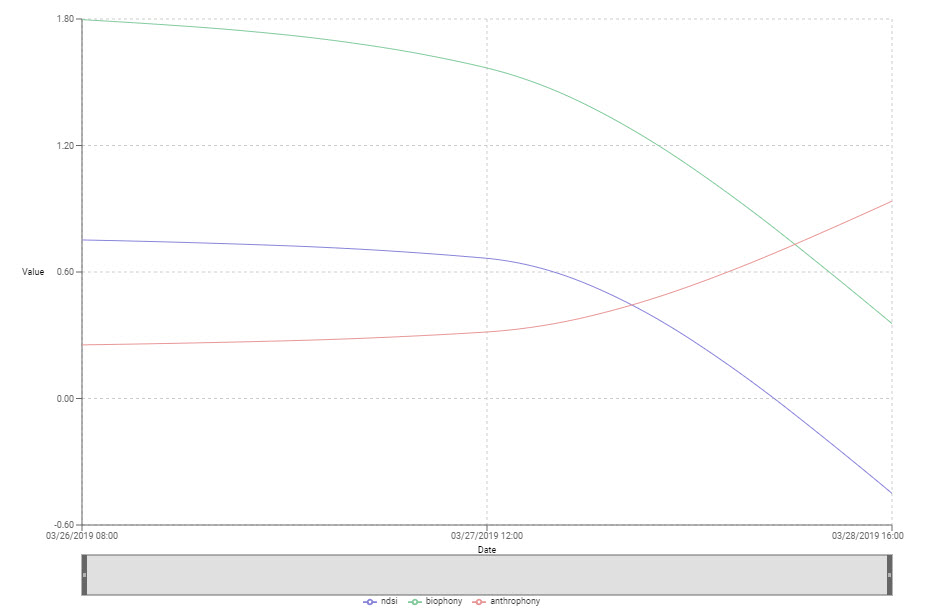
\includegraphics[width=\textwidth]{NDSIgraph3} \\[12pt]
\end{center}
The line graphs available for NDSI value show the NDSI, anthrophony, and biophony by date and time. Researchers often record at different times of day in order to see how index values compare through out the day.\par

\begin{center}
  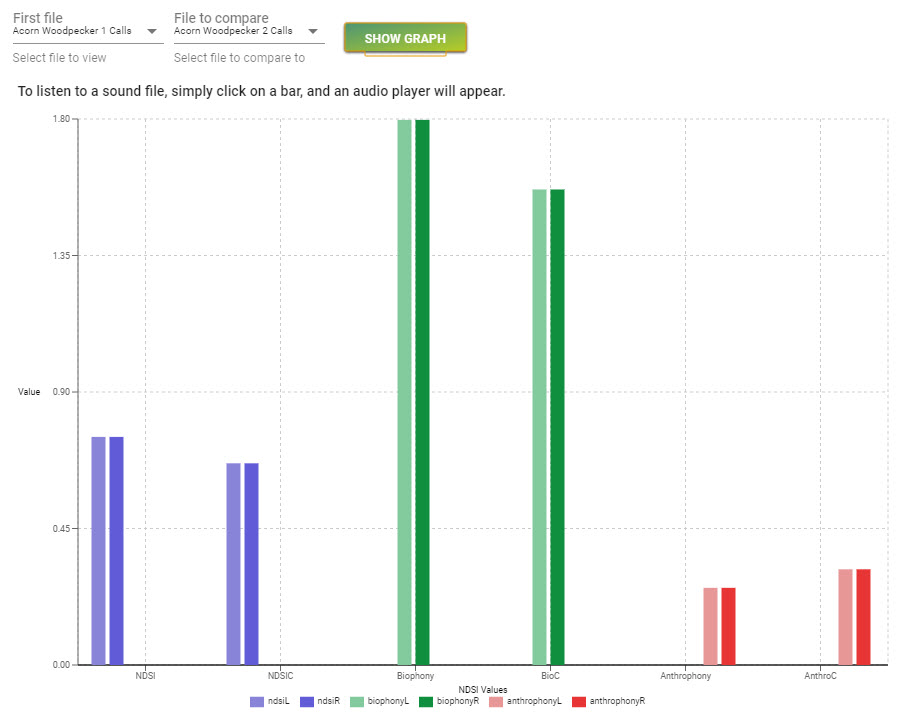
\includegraphics[width=\textwidth]{NDSIgraph4} \\[12pt]
\end{center}
This graph is used to view any individual file in the selected Site and/or Series. This allows for a closer look at what is going on in the data, and also allows you to compare them to other files in the data set, as seen in the image above. With this graph, the user can select a bar chart and an audio player will appear for the user to listen to that file in the client.

/\subsection{Acoustic Complexity Index}
\par The emerging field of soundscape ecology focuses on using the sounds in an environment to analyze, predict and correct the problems within that environment. These problems are often caused by the ever-present human expansion into previously undisturbed natural habitats. This invasion of habitats means that the organisms that live there are constantly forced leave due to the increase in human made machine noise (Anthrophony). This Anthrophony disrupts the organism's natural communication, since most organisms rely on sound to communicate. Those organisms that choose to stay and overcome the noise leave a sonic footprint within the environment itself. Often this footprint can tell a story about the troubles with biodiversity in an area. This is where the Acoustic Complexity Index or ACI comes into play. First used in Tuscan Emilian Apennine National Park, Italy; The ACI measures the change in acoustic intensity. This allows for researchers to pinpoint areas of interesting sound within a recording, even through human made machine noise or Anthrophony. Allowing for research of the biodiversity in areas that have been tainted with human sound.
\begin{center}
  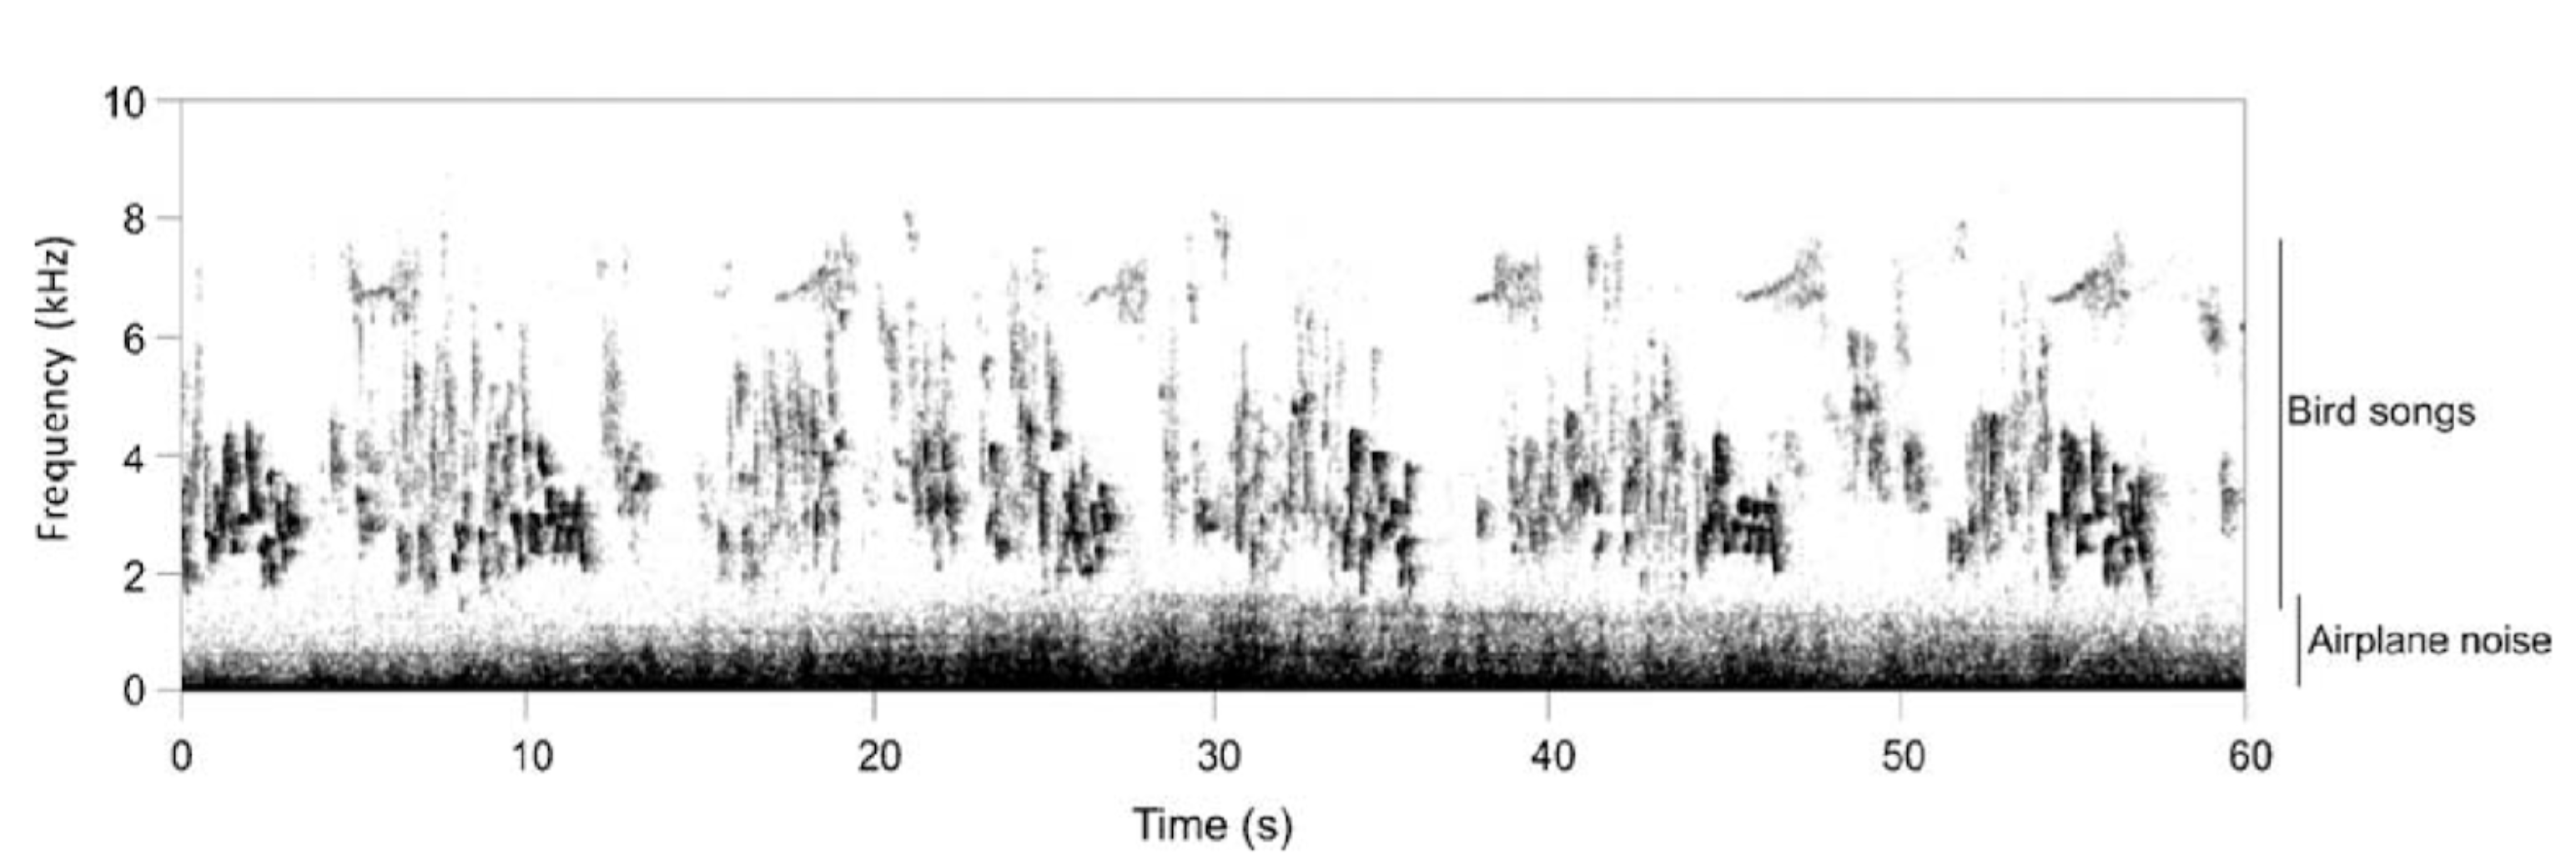
\includegraphics[width=0.85\textwidth]{ACI} \\[12pt]
\end{center}
\par ACI relies on the fact that most Biophonic (non-human biological sounds) have a high level of complexity when it comes to their intensity. Meaning that most natural sounds have a high variance of loudness. This is in stark contrast with the mostly monotone nature of human made sounds. This key difference in sound types allows the ACI to filter out plane noises or car sounds amongst bird sounds and other Biophonic interests. When compared to the previous technique of cutting off at certain sound frequency indexes, the ACI tends to save useful data from being truncated and lost.
\par During a trial done by N. Pieretti the ACI was shown to have a high correlation with the number of bird vocalizations in an area. This comparison was done by placing 20 digital recorders 100m apart in a 4x5 grid in the previously mentioned Italian park. Areas that were recorded to have high levels of bird sound also had a correlated high ACI.
\begin{quote}
 ``The strong correlation between the ACI and the singing activity of the avian community
  is related to the capacity of this index to successfully highlight rapid variations of the
  intensity in each single frequency bin, a feature that is typical of bird songs.''\cite{pieretti}
\end{quote}

Increasing the length of sound track that was analyzed also increased in a correlation between ACI and number of bird vocalizations.

\begin{center}
  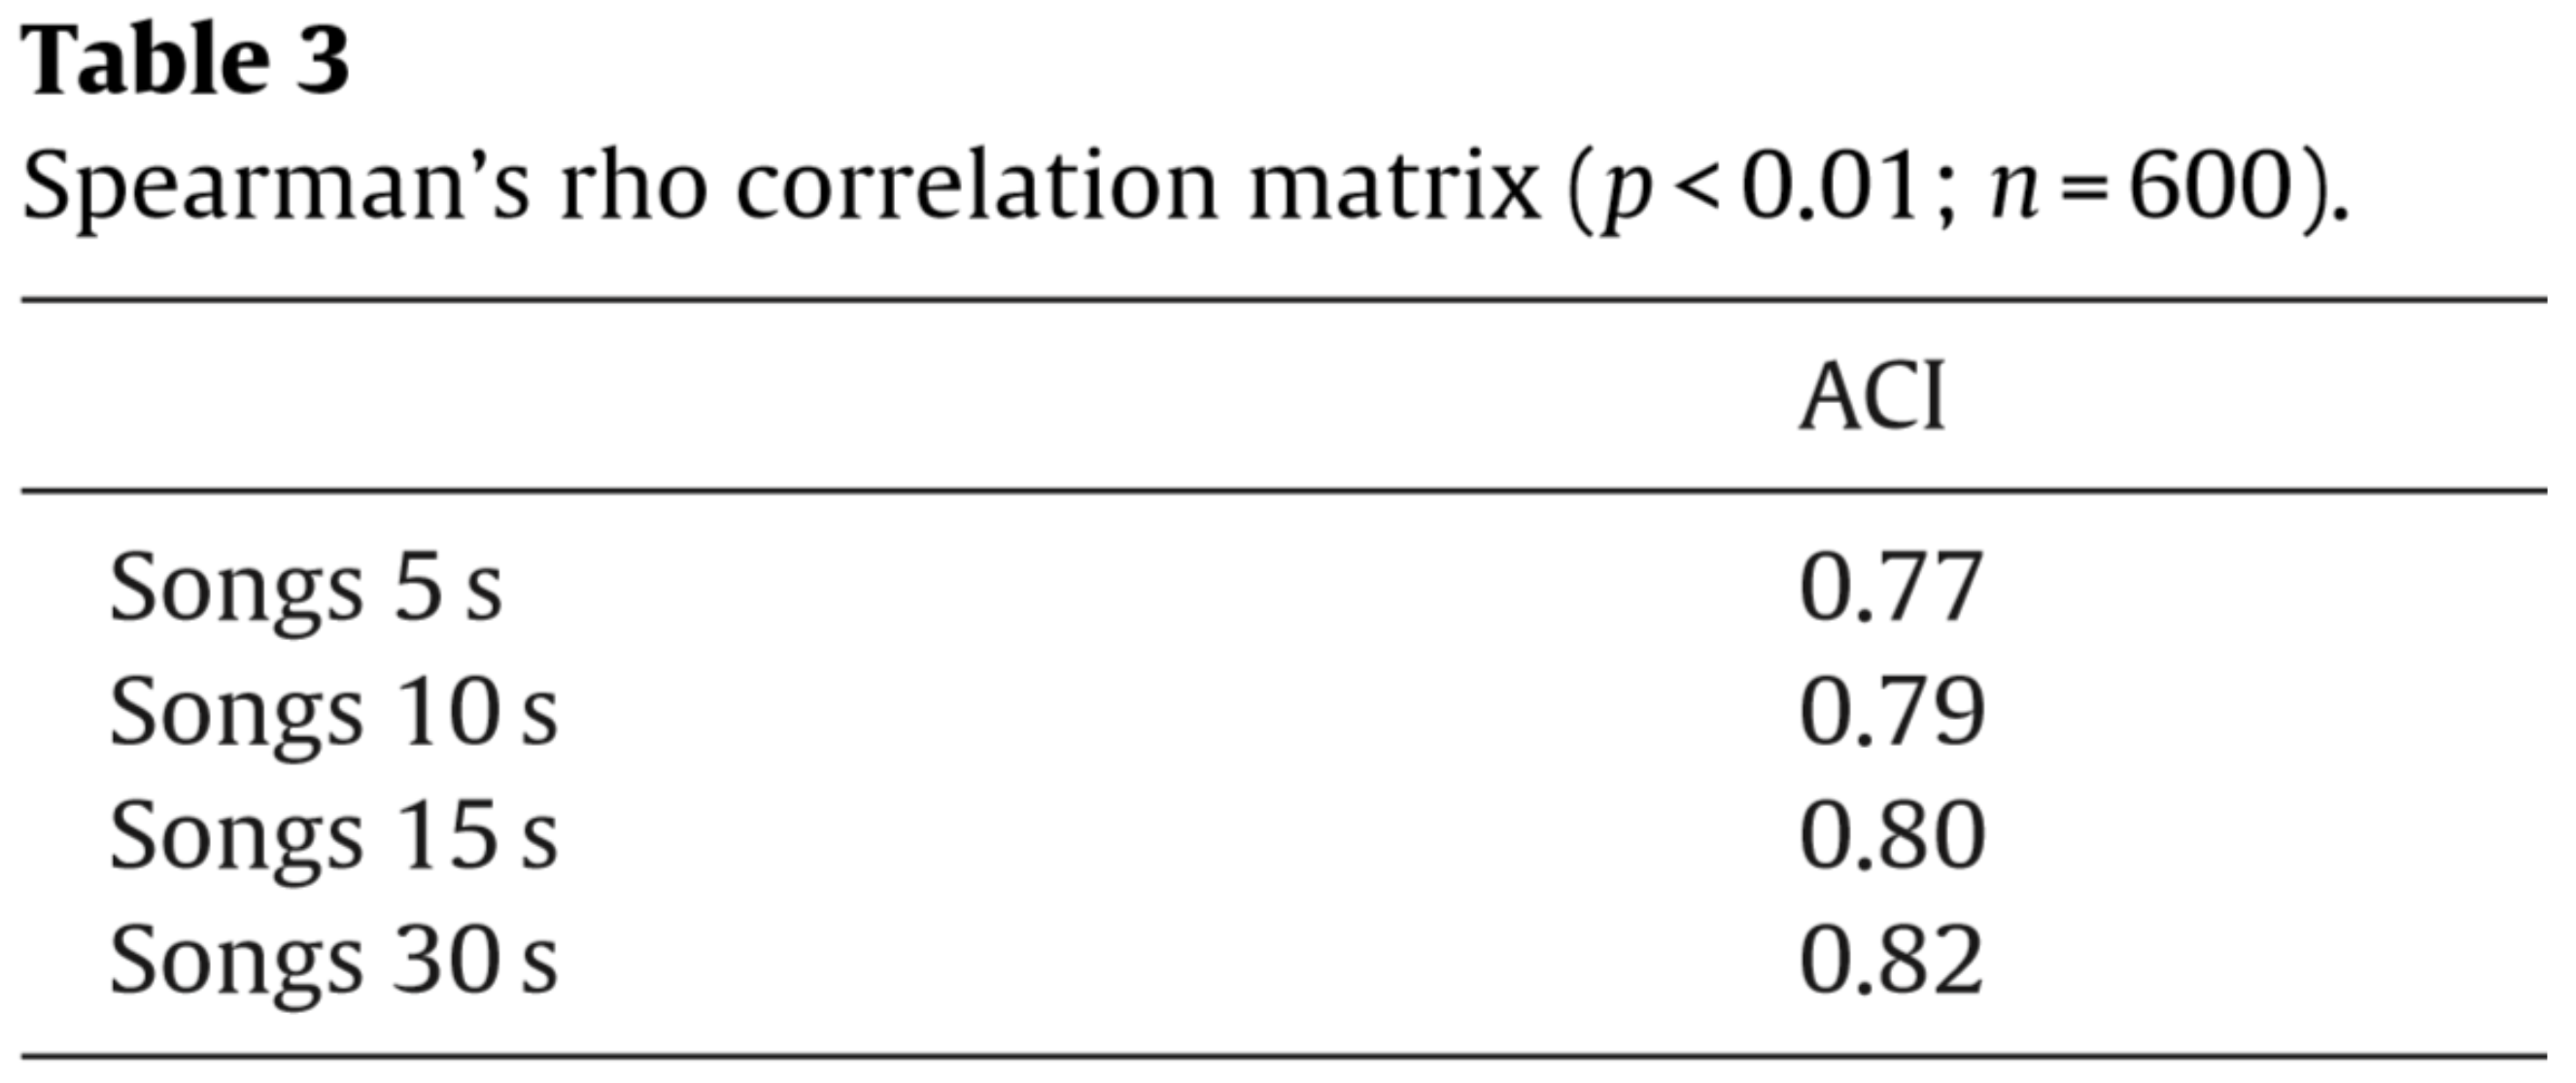
\includegraphics[width=0.85\textwidth]{RhoCorrelation} \\[12pt]
\end{center}

\par While there is a promising amount of research for the ability of the ACI to discriminate between Anthrophony and Biophony, the algorithm still does very poorly in discerning between different types of Biophony and Geophony. This challenge can be highlighted by the fact that the algorithm produces high numbers for sounds such as buzzing insects and wind. Both of which have high variance of intensity and thus increase the ACI value for a given sound bucket. Along this same strain of problem, the ACI cannot differentiate between species or even types of animal sounds. This type of classification is still left up to techniques such as model recognizers; models that are built to recognize one type of species. In the study, the Wildlife Acoustics program was used to build these recognition models and provide a benchmark for the accuracy of the ACI.
\par The ACI, in combination with other measuring techniques, can be a powerful tool for finding the Biophonic sounds within a recording. These types of breakthroughs in soundscape ecology allow professional Ornithologists to conduct research efficiently without ever having to travel into the field. Hopefully our Senior Design project will allow researchers and other interested individuals to access these algorithms and use them to analyze the effects of human made sounds on the surrounding habitats.\cite{pieretti}

\input{soundecology/visualizations/adiaei}
\subsubsection{Bioacoustic Index Visualization}
For the Bioacoustic index, the value output by the algorithms is an area value under a curve for both the left and right channels where relevant. Thus initially, the best representation of this index would be a stacked area graph, with both the left and right channels included.\\

\begin{center}
	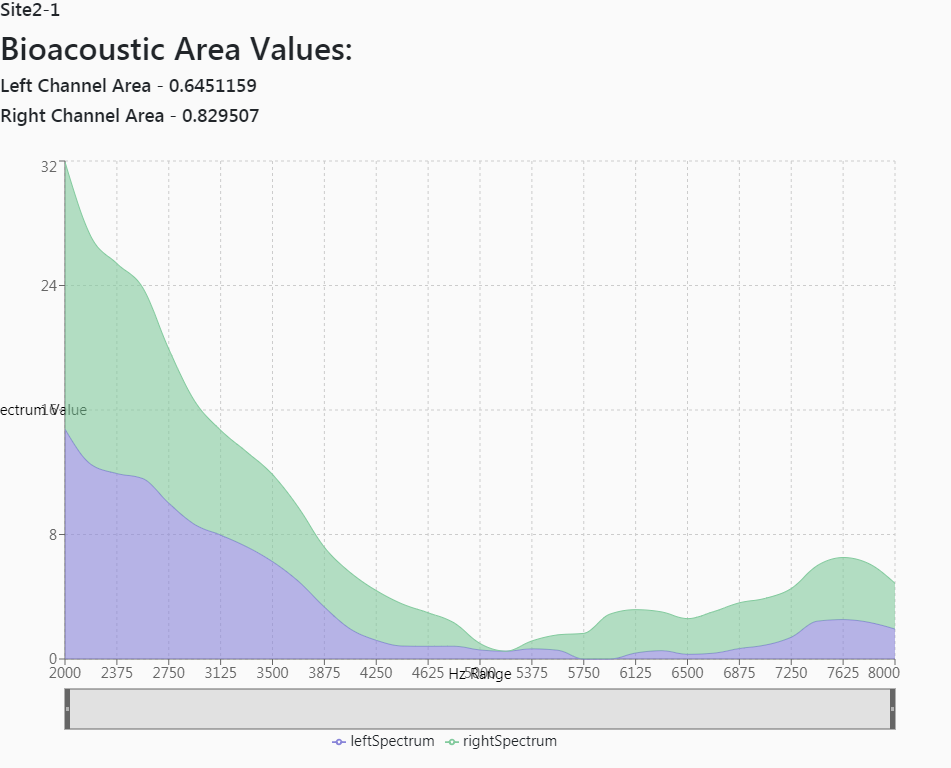
\includegraphics[width=\textwidth]{BAgraph1} \\[12pt]
\end{center}
This graph includes both channels, with a brush included much like in ACI. Because the index calculates a literal area under a curve, an area chart is logically the best representation, and the graphic helps to support this. Again, the user can filter by hertz range using the brush, giving insight into the values in specific ranges. This particular graph is comparing two files in from the same site, but different series. This helps to show the distinct difference in BI values between the two.\\

\subsubsection{RMS Visualization}
NEED TO PUT EXPLANATION OF RMS HERE

\begin{center}
  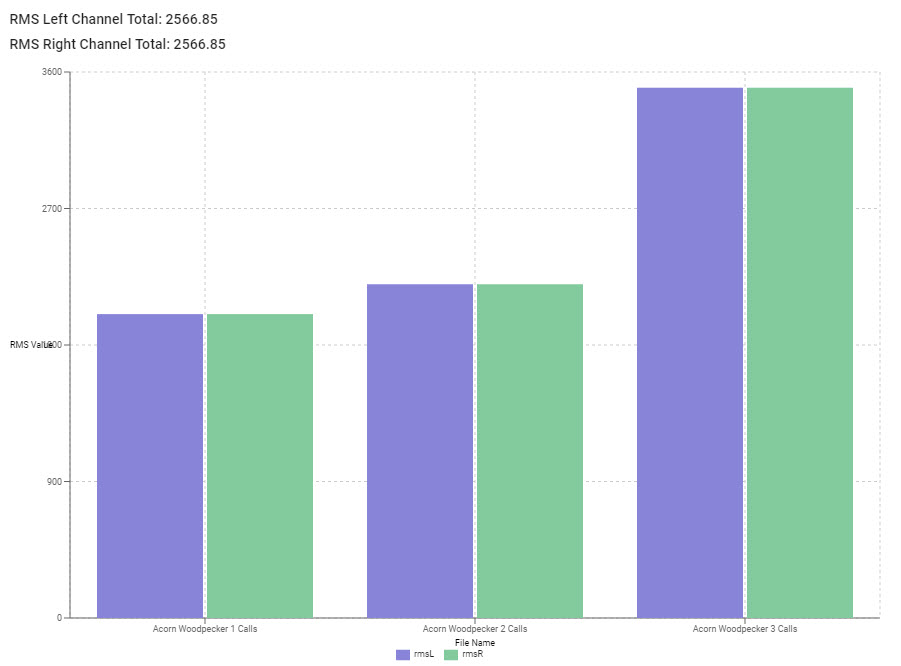
\includegraphics[width=\textwidth]{RMSgraph1} \\[12pt]
\end{center}
As RMS is a single value output, it is best to just display those values for each channel, and use a simple bar chart to represent them visually.

\subsubsection{Comparing Data Sets and Files}
Comparing data sets is maybe the most important feature of this service. In doing this, a researcher can evaluate index values over time, using different data sets for different things. For example, a researcher may be working in a site, recording data in the morning and at night, every day for a week. The researcher would process both sets separately using whichever indices and parameters they wish, and name and tag the sets appropriately. Then, in the Catalog, they can select both data sets, and see visualizations comparing the two sets across time, to see how the index values match up on the same days but in the morning and at night.\par
From a research perspective, this is the best way to draw conclusions from the indices included in this service, as the more data that is collected and processed, the more sense they make. An example of this includes a forest where human interaction is on the rise. Using an index like ACI over time will help to make correlations as to how human invasion on the forest is affecting the wildlife. Alternatively, for comparing across sites, if a species of animal is found in multiple locations, the ACI index can be used to roughly determine the number of these species in the area. Comparing this value across the sites is useful for determining species population in different areas.\\

\begin{center}
	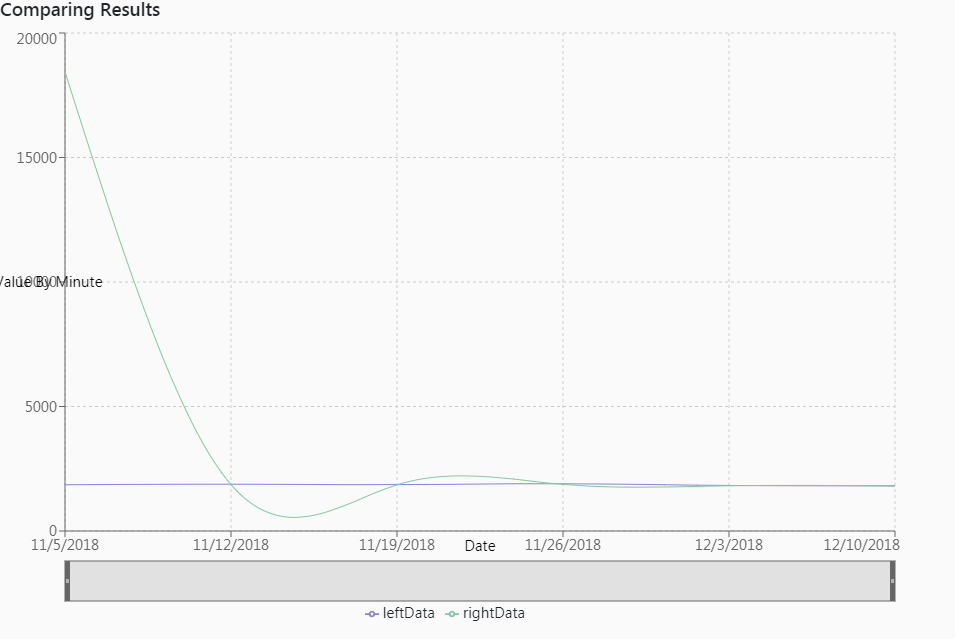
\includegraphics[width=\textwidth]{CompareACIgraph1} \\[12pt]
	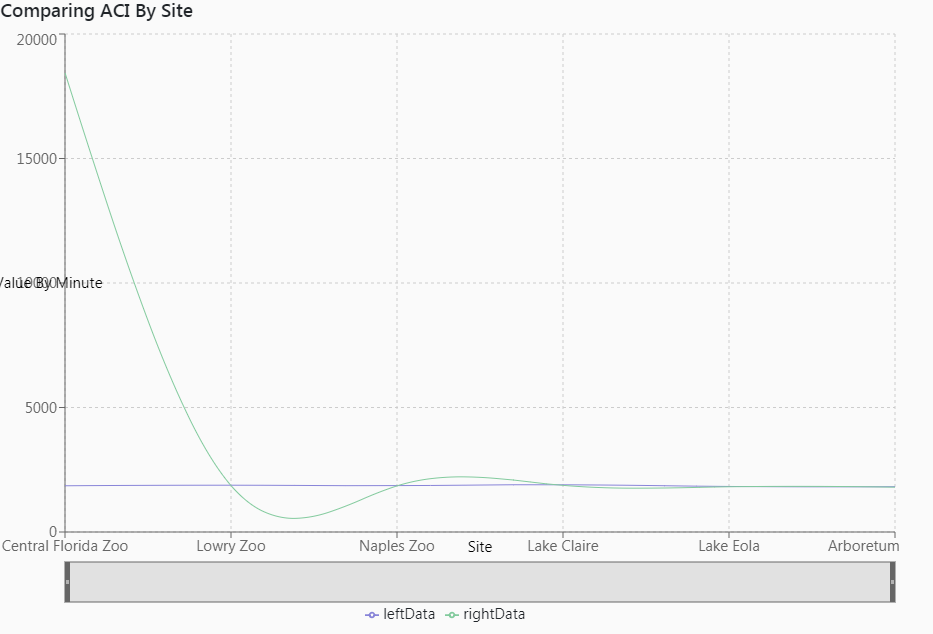
\includegraphics[width=\textwidth]{CompareACIgraph2} \\[12pt]
\end{center}

The first is a comparison graphic for ACI index across time. The data used was six files, all recorded a week apart. The X axis represents the date of each file, and the Y axis shows the ACI value by minute for each date. The other comparison available for ACI is comparing across data sites. Much like the other ACI comparison graph, the Y axis again shows the ACI value by minute, while the X axis for this graph represents the site. Overall, these two comparison charts give the researcher two different comparison insights for the ACI index.\\

\begin{center}
	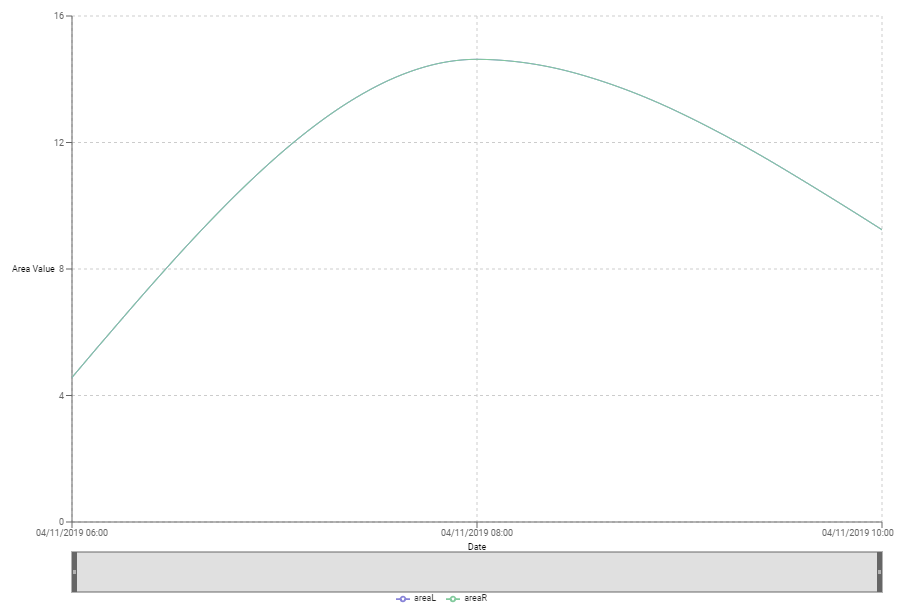
\includegraphics[width=\textwidth]{CompareBAgraph1} \\[12pt]
	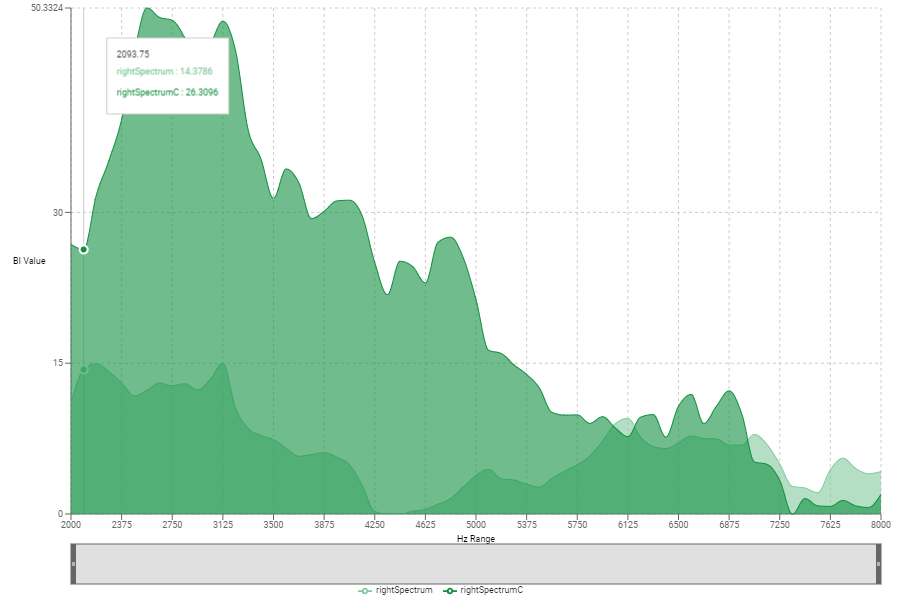
\includegraphics[width=\textwidth]{CompareBAgraph2} \\[12pt]
\end{center}

These two graphs represent the comparison charts available for the Bioacoustic Index. Again, the user has comparison across dates and research sites available to them. The brush is included to allow the user to shorten the observed time range as they please.\\

\begin{center}
	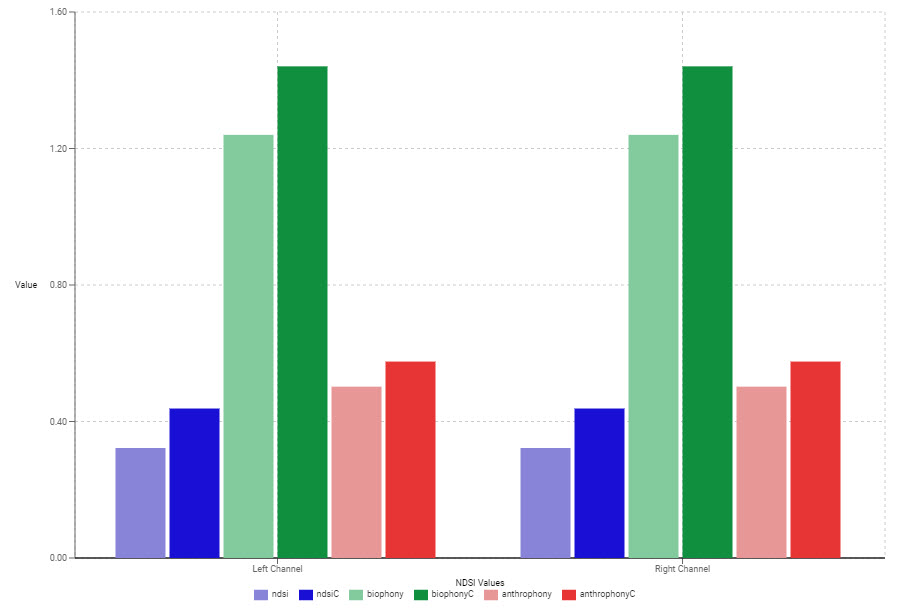
\includegraphics[width=\textwidth]{CompareNDSIgraph1} \\[12pt]
	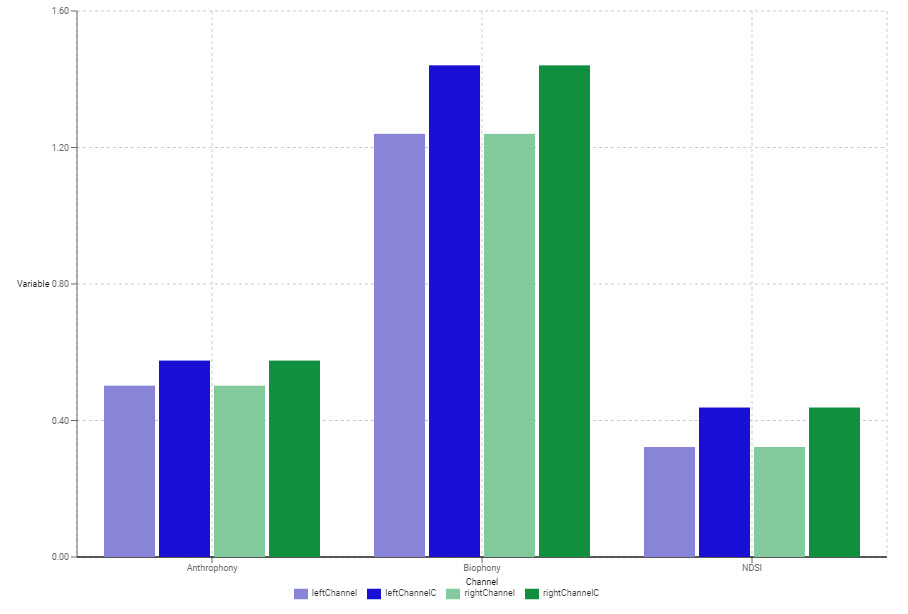
\includegraphics[width=\textwidth]{CompareNDSIgraph2} \\[12pt]
\end{center}

The NDSI index includes three different variables of interest to the user. These two images show the biophony comparison across date and the NDSI comparison across sites respectively. These charts are bar graphs to show the respective value by channel, along with a line that helps to show the change intensity between values. Notice that the NDSI is upside down, this is because NDSI values are typically negative due to the nature of the index. A brush is included as per usual.\\

\begin{center}
	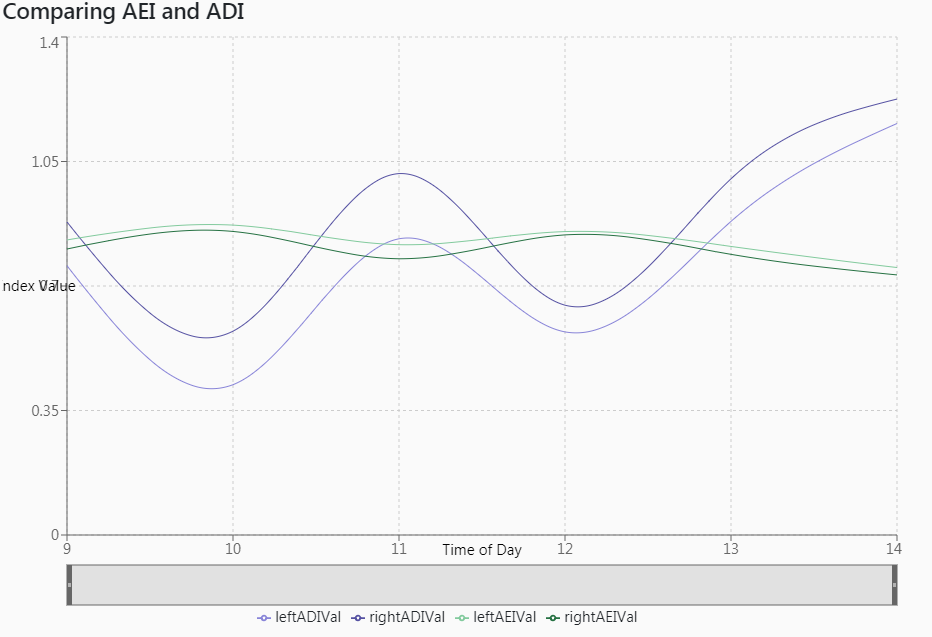
\includegraphics[width=\textwidth]{ADIAEIgraph1} \\[12pt]
\end{center}
ADI and AEI indices are closely related, thus it is useful for the user to be able to view them side by side. In the graphs available, as long as a data set has had both ADI and AEI run on it, the user will have the option to view the AEI and ADI data individually, as shown in their respective section, but also side by side, as seen above. This graph shows the ADI and AEI values for each channel over the time of day they were recorded. They are color coded to show their relationship to one another by channel, and contrast each other by index. A brush is also included.

